% Options for packages loaded elsewhere
% Options for packages loaded elsewhere
\PassOptionsToPackage{unicode}{hyperref}
\PassOptionsToPackage{hyphens}{url}
\PassOptionsToPackage{dvipsnames,svgnames,x11names}{xcolor}
%
\documentclass[
  authoryear,
  preprint,
  3p]{elsarticle}
\usepackage{xcolor}
\usepackage{amsmath,amssymb}
\setcounter{secnumdepth}{5}
\usepackage{iftex}
\ifPDFTeX
  \usepackage[T1]{fontenc}
  \usepackage[utf8]{inputenc}
  \usepackage{textcomp} % provide euro and other symbols
\else % if luatex or xetex
  \usepackage{unicode-math} % this also loads fontspec
  \defaultfontfeatures{Scale=MatchLowercase}
  \defaultfontfeatures[\rmfamily]{Ligatures=TeX,Scale=1}
\fi
\usepackage{lmodern}
\ifPDFTeX\else
  % xetex/luatex font selection
\fi
% Use upquote if available, for straight quotes in verbatim environments
\IfFileExists{upquote.sty}{\usepackage{upquote}}{}
\IfFileExists{microtype.sty}{% use microtype if available
  \usepackage[]{microtype}
  \UseMicrotypeSet[protrusion]{basicmath} % disable protrusion for tt fonts
}{}
\makeatletter
\@ifundefined{KOMAClassName}{% if non-KOMA class
  \IfFileExists{parskip.sty}{%
    \usepackage{parskip}
  }{% else
    \setlength{\parindent}{0pt}
    \setlength{\parskip}{6pt plus 2pt minus 1pt}}
}{% if KOMA class
  \KOMAoptions{parskip=half}}
\makeatother
% Make \paragraph and \subparagraph free-standing
\makeatletter
\ifx\paragraph\undefined\else
  \let\oldparagraph\paragraph
  \renewcommand{\paragraph}{
    \@ifstar
      \xxxParagraphStar
      \xxxParagraphNoStar
  }
  \newcommand{\xxxParagraphStar}[1]{\oldparagraph*{#1}\mbox{}}
  \newcommand{\xxxParagraphNoStar}[1]{\oldparagraph{#1}\mbox{}}
\fi
\ifx\subparagraph\undefined\else
  \let\oldsubparagraph\subparagraph
  \renewcommand{\subparagraph}{
    \@ifstar
      \xxxSubParagraphStar
      \xxxSubParagraphNoStar
  }
  \newcommand{\xxxSubParagraphStar}[1]{\oldsubparagraph*{#1}\mbox{}}
  \newcommand{\xxxSubParagraphNoStar}[1]{\oldsubparagraph{#1}\mbox{}}
\fi
\makeatother


\usepackage{longtable,booktabs,array}
\newcounter{none} % for unnumbered tables
\usepackage{calc} % for calculating minipage widths
% Correct order of tables after \paragraph or \subparagraph
\usepackage{etoolbox}
\makeatletter
\patchcmd\longtable{\par}{\if@noskipsec\mbox{}\fi\par}{}{}
\makeatother
% Allow footnotes in longtable head/foot
\IfFileExists{footnotehyper.sty}{\usepackage{footnotehyper}}{\usepackage{footnote}}
\makesavenoteenv{longtable}
\usepackage{graphicx}
\makeatletter
\newsavebox\pandoc@box
\newcommand*\pandocbounded[1]{% scales image to fit in text height/width
  \sbox\pandoc@box{#1}%
  \Gscale@div\@tempa{\textheight}{\dimexpr\ht\pandoc@box+\dp\pandoc@box\relax}%
  \Gscale@div\@tempb{\linewidth}{\wd\pandoc@box}%
  \ifdim\@tempb\p@<\@tempa\p@\let\@tempa\@tempb\fi% select the smaller of both
  \ifdim\@tempa\p@<\p@\scalebox{\@tempa}{\usebox\pandoc@box}%
  \else\usebox{\pandoc@box}%
  \fi%
}
% Set default figure placement to htbp
\def\fps@figure{htbp}
\makeatother





\setlength{\emergencystretch}{3em} % prevent overfull lines

\providecommand{\tightlist}{%
  \setlength{\itemsep}{0pt}\setlength{\parskip}{0pt}}



 
\usepackage[]{natbib}
\bibliographystyle{elsarticle-harv}


\makeatletter
\@ifpackageloaded{caption}{}{\usepackage{caption}}
\AtBeginDocument{%
\ifdefined\contentsname
  \renewcommand*\contentsname{Table of contents}
\else
  \newcommand\contentsname{Table of contents}
\fi
\ifdefined\listfigurename
  \renewcommand*\listfigurename{List of Figures}
\else
  \newcommand\listfigurename{List of Figures}
\fi
\ifdefined\listtablename
  \renewcommand*\listtablename{List of Tables}
\else
  \newcommand\listtablename{List of Tables}
\fi
\ifdefined\figurename
  \renewcommand*\figurename{Figure}
\else
  \newcommand\figurename{Figure}
\fi
\ifdefined\tablename
  \renewcommand*\tablename{Table}
\else
  \newcommand\tablename{Table}
\fi
}
\@ifpackageloaded{float}{}{\usepackage{float}}
\floatstyle{ruled}
\@ifundefined{c@chapter}{\newfloat{codelisting}{h}{lop}}{\newfloat{codelisting}{h}{lop}[chapter]}
\floatname{codelisting}{Listing}
\newcommand*\listoflistings{\listof{codelisting}{List of Listings}}
\makeatother
\makeatletter
\makeatother
\makeatletter
\@ifpackageloaded{caption}{}{\usepackage{caption}}
\@ifpackageloaded{subcaption}{}{\usepackage{subcaption}}
\makeatother
\journal{Fisheries Research}
\usepackage{bookmark}
\IfFileExists{xurl.sty}{\usepackage{xurl}}{} % add URL line breaks if available
\urlstyle{same}
\hypersetup{
  pdftitle={Mismatched Maturity: The Sensitivity of the Gulf of Alaska Northern Rockfish Assessment to Unaccounted Skip Spawning},
  pdfauthor={Benjamin C. Williams},
  pdfkeywords={skip spawning, northern rockfish, stock
assessment, spawning stock biomass},
  colorlinks=true,
  linkcolor={blue},
  filecolor={Maroon},
  citecolor={Blue},
  urlcolor={Blue},
  pdfcreator={LaTeX via pandoc}}


\setlength{\parindent}{6pt}
\begin{document}

\begin{frontmatter}
\title{Mismatched Maturity: The Sensitivity of the Gulf of Alaska
Northern Rockfish Assessment to Unaccounted Skip Spawning}
\author[1]{Benjamin C. Williams%
%
}
 \ead{ben.williams@noaa.gov} 

\affiliation[1]{organization={Auke Bay Laboratories, Alaska Fisheries
Science Center, National Marine Fisheries Service, National Oceanic and
Atmospheric Administration},addressline={17109 Point Lena Loop
Rd.},city={Juneau, Alaska},postcode={99801, USA},postcodesep={}}

\cortext[cor1]{Corresponding author}

        
\begin{abstract}
Accurate estimation of spawning stock biomass is foundational to
sustainable fisheries management, yet fishery assessments often assume
equivalence between biological maturity (physiological capacity) with
functional maturity (active spawning). This study utilizes an
RTMB-based, closed-loop simulation to evaluate the management
implications of unaccounted skip spawning for the Gulf of Alaska
northern rockfish (\emph{Sebastes polyspinis}) stock. An integrated,
age-structured operating model governed by functional maturity was
simulated to compare a ``matched'' assessment scenario against a
``mismatched'' scenario that bases reference points on biological
maturity. Under the North Pacific Fisheries Management Council Tier 3
Harvest Control Rule, variations in maturity definitions inherently
shift per-recruit reference points (e.g., \(F_{40}\)). Results
illustrate how this structural difference influences estimates of
reproductive resilience and perceived stock status relative to the
operating model, which vary with differing levels of skip spawning at
age.
\end{abstract}





\begin{keyword}
    skip spawning \sep northern rockfish \sep stock assessment \sep 
    spawning stock biomass
\end{keyword}
\end{frontmatter}
    

\section{Introduction}\label{introduction}

In data-moderate or data-rich, age-structured fishery stock assessments
maturity is typically treated as a determinist and often time invariant
input \citep{Miller2018}. The maturity ogive, which defines the
proportion of individuals mature at a given age or length, is generally
estimated externally to the assessment model. This is frequently
achieved using logistic regression to fit histological or macroscopic
data from scientific surveys \citep{Williams2016}. Within this
framework, the annual female spawning stock biomass (SSB) serves as the
primary proxy for the stock's reproductive potential. SSB is calculated
as the sum product of the number of females-at-age, their average or
annual weight-at-age, and the proportion mature-at-age. This metric
relies on the assumption of proportionality
\citep{Morgan2008, Lambert2008}, that mature female biomass is linearly
related to total egg production (TEP) and by extension, expected
recruitment of the stock.

However, the validity of SSB as a proxy for reproductive output depends
heavily on how maturity is defined and quantified. As highlighted by
\citet{Head2020}, there is a fundamental distinction between biological
maturity and functional maturity. Biological maturity refers to the
developmental milestone where an individual becomes physiologically
capable of producing gametes (i.e., the anatomical presence of developed
gonads). Functional maturity, refers to the proportion of biologically
mature individuals that actually contribute to a spawning event. The
discrepancy between these two measures is primarily driven by ``skip
spawning'', a life-historystrategy where biologically mature adults
forgo reproduction to prioritize somatic growth or survival
\citep{Jorgensen2006, Secor2008}. When assessments rely soley on
biological maturity in the presence of skip spawning, they risk
overestimating the effective spawning biomass and distorting the
resultant biological reference points.

Despite its prevalence \citep{Jorgensen2006, Secor2008, Rideout2011},
skip spawning has rarely been explicitly modeled in stock assessments.
Traditional macroscopic maturity staging often fails to distinguish
between skip-spawners from immature individuals
\citep{Rodgveller2018, McBride2022}, or simply lumps all large fish into
a mature category. When an assessment attributes reproductive output to
non-spawning individuals, it can create a ``productivity illusion''
where the model observes a high spawning biomass producing average
recruitment and incorrectly infers that the stock has low intrinsic
productivity (e.g., low steepness).

The implications of this misspecification extend beyond biological
accuracy to the core of management performance. While \citet{Secor2008}
noted that misspecified reproductive schedules could bias biological
reference points (such as \(F_{MSY}\) or \(F_{40\%}\)), few studies have
quantified how this specific biological error propagates through a
harvest control rule (HCR). It remains unclear whether the resulting
management advice is inherently risky, leading to overfishing or
unintentionally precautionary, leading to foregone yield.

To address this gap, a simulation testing framework was developed for
northern rockfish (\emph{Sebastes polyspinis}) in the Gulf of Alaska
(GOA) as a case study. Northern rockfish are a long-lived, ovoviviparous
\citep{Kendall1987}, and known to exhibit skip spawning
\citep{Conrath2019}. They support a directed fishery, and are managed
using an integrated age-structured stock assessment that assumes
biological maturity \citep{Williams2023}. To evaluate the sensitivity of
the GOA northern rockfish stock assessment to unaccounted skip spawning,
a simulation testing framework was developed. This framework relies on
an age-structured, single-sex operating model (OM) parameterized with
skip spawning dynamics to generate synthetic observation data with
realistic error. This OM is coupled with an estimation model (EM) within
a feedback loop to simulate the annual stock assessment and management
process using the North Pacific Fisheries Management Council (NPFMC)
Tier 3 HCR \citep{Dorn2020}. By comparing scenarios where the EM
correctly accounts for functional maturity against a misspecified those
relying on biological maturity, this study evaluates the sensitivity of
stock status estimates and management performance to maturity
misspecification.

\section{Methods}\label{methods}

\subsubsection{Biological and Functional
Maturity}\label{biological-and-functional-maturity}

Historical age-at-maturity for northern rockfish was based on a logistic
curve fitted to ovarian samples from 1996 (n=75) and 2000--2001 (n=157)
\citep{Heifetz2003, Chilton2007}. These data were integrated with
contemporary samples (n=274) that explicitly identified skip-spawning
events via histological analysis \citep{Conrath2019}.

Biological maturity (\(M_{b,a}\)) was estimated using a binomial
Generalized Linear Model (GLM) with a logit link in R \citep{Rcore}. To
account for limited sampling of juvenile age classes and ensure the
ogive approached zero at younger ages, observations for fish \(\le\)
age-6 were assigned higher weights in the likelihood function
\citep{Conrath2021}. Because maturity with skip-spawning exhibits
non-logistic (Type IV) distributions \citep{Trippel1991}, the
age-specific probability of skip spawning (\(P_{skip,a}\))\$ was modeled
independently using a binomial Generalized Additive Model (GAM) with a
cubic regression spline for age, implemented via the mgcv package in R
\citep[\citet{Rcore}]{mgcv}. Observed functional maturity (\(M_{f,a}\)),
representing the proportion of the population contributing to spawning,
was calculated by adjusting the biological ogive by :
\begin{equation}\protect\phantomsection\label{eq-pskip}{
M_{f,a} = M_{b,a} \times (1 - P_{skip,a}).
}\end{equation}

\subsection{Simulation Framework (Operating
Model)}\label{simulation-framework-operating-model}

\subsubsection{Simulated Skip-Spawning
Scenarios}\label{simulated-skip-spawning-scenarios}

To evaluate the sensitivity of the assessment model across a range of
unobserved dynamics, 18 distinct skip-spawning scenarios were simulated
(6 functional shapes X 3 maximum intensities: 10\%, 20\%, and 30\%).
Because empirical observations of northern rockfish skip spawning are
limited across the full age structure of a population, and are unknown
both temporally and spatially in the GOA, this approach allowed for the
exploration of diverse functional forms and intensities. Age-specific
skip-spawning probabilities, \(P_{skip,a}\), were simulated using a
flexible curve-generating algorithm between ages 3--50, assuming no skip
spawning outside this range. The functional shapes included:

\begin{itemize}
\tightlist
\item
  Dome/Skewed Dome: A symmetric, Gaussian-like curve where skip spawning
  peaks at the intermediate or early-mature ages.
\item
  Inverse Dome: High skipping in young and old individuals, low in
  middle ages.
\item
  Linear (Increasing/Decreasing): Constant change in skipping
  probability.
\item
  Constant: A uniform rate applied equally to all ages.
\end{itemize}

\begin{figure}

\centering{

\includegraphics[width=4.33in,height=\textheight,keepaspectratio]{../figs/skip.png}

}

\caption{\label{fig-skip}Simulated skip spawning-at-age and resultant
functional maturity ogives. The observed functional ogive (From the data
presented in Conrath, 2019) is shown in light gray in the right side
panes.}

\end{figure}%

\subsubsection{Population Dynamics}\label{population-dynamics}

A closed-loop simulation framework, conceptually similar to a management
strategy evaluation \citep[MSE,][]{Punt2016}, was used to evaluate the
management implications of skip spawning for northern rockfish in the
GOA. This framework couples a biological OM, which simulates the
``true'' population dynamics using functional maturity, to an EM that
mimics the current stock assessment and HCR process. The simulation
operates as an age-structured, single-sex, single-region, single-fishery
population model projected at annual time steps. The abundance of
individuals of age \(a\) in year \(y\), denoted as \(N_{a,y}\), is
projected forward using standard exponential decay dynamics with
parameter inputs taken from the most recent full fishery assessment
\citep{Williams2023}.

Total mortality (\(Z_{a,y}\)) is partitioned into natural mortality
(\(M\)) and fishing mortality (\(F_y\)), modulated by age-specific
fishery selectivity (\(s^{f}_a\)):

\begin{equation}\protect\phantomsection\label{eq-tot-mort}{
Z_{a,y} = M + F_y s^{f}_a
}\end{equation}

Survival and abundance for ages between the recruitment age
(\(a_{min}\)) and the plus-group age (\(A\)) follow:

\begin{equation}\protect\phantomsection\label{eq-Nat}{N_{a,y} = \begin{cases} 
R_{y} & \text{for } a = a_{min} \\ 
N_{a-1,y} e^{-Z_{a-1,y-1}} & \text{for } a_{min} < a < A \\ 
N_{A-1,y} e^{-Z_{A-1,y-1}} + N_{A,y-1} e^{-Z_{A,y-1}} & \text{for } a = A \text{ (Plus Group)} 
\end{cases}
}\end{equation}

Annual recruitment (\(R_y\)) serves as the primary source of stochastic
variability between simulations. Three specific recruitment scenarios
were evaluated with future recruitment generated stochastically by
drawing from log-normal distributions parameterized using quantiles of
estimated historical log-recruitment from the assessment
\citep{Williams2023}.

Three recruitment scenarios were explored, median recruitment, a crash
recruit (5th quantile for 20 years, followed by 80th quantile), and high
recruitment (80th quantile).

\begin{itemize}
\tightlist
\item
  \emph{Average:} Median historical log-recruitment with a log-standard
  deviation of 0.2.
\item
  \emph{High:} 80th quantile historical log-recruitment with a
  log-standard deviation of 0.2.
\item
  \emph{Crash:} 5th quantile historical log-recruitment with a
  log-standard deviation of 0.1 for 20 years, followed by 80th quantile
  historical log-recruitment with a log-standard deviation of 0.2 for
  the remaining years.
\end{itemize}

Catch in numbers at age (\(C_{a,y}\)) is calculated using the Baranov
catch equation \citep{Branch2009}:

\begin{equation}\protect\phantomsection\label{eq-catch}{
C_{a,y} = \frac{F_y s^{f}_a}{Z_{a,y}} N_{a,y} (1 - e^{-Z_{a,y}})
}\end{equation}

Total yield (\(Y_y\)) is the sum product of catch numbers and weight
(\(W_a\)):

\begin{equation}\protect\phantomsection\label{eq-yield}{
Y_y = \sum_{a} C_{a,y} W_a
}\end{equation}

\subsection{Defining the Biological
Mismatch}\label{defining-the-biological-mismatch}

A core component of this study is the distinction between annual
biological and functional \(SSB_y\). It is calculated at a specific
spawning fraction of the year (\(\phi_{spawn}\)), adjusting for
mortality prior to spawning:

\begin{equation}\protect\phantomsection\label{eq-ssb}{
SSB_y = \sum_{a=a_{min}}^{A} N_{a,y} e^{-Z_{a,y} \cdot \phi_{spawn}} \cdot W_a \cdot \Phi_{a,y}
}\end{equation}

To quantify the cost of misspecification, the model defines the maturity
ogive \(\Phi_{a,y}\) differently depending on the scenario:

\emph{Functional Maturity (\(\Phi^{func}_{a,y}\)):} Represents the
realized proportion of individuals that actually spawn, accounting for
skip spawning rates (\(P_{skip, a}\)). This is the ``true'' state used
in the OM and the correctly specified EM.

\begin{equation}\protect\phantomsection\label{eq-func-mat}{
\Phi^{func}_{a,y} = \Phi^{bio}_{a} \cdot (1 - P_{skip, a})
}\end{equation}

\emph{Biological Maturity (\(\Phi^{bio}_{a}\)):} Represents the
proportion of individuals physiologically capable of reproduction. This
vector is used in the misspecified EM.

\begin{equation}\protect\phantomsection\label{eq-bio-mat}{
\Phi^{bio}_{a} = \frac{1}{1 + e^{-\frac{a - a_{50}}{k}}}
}\end{equation}

\subsection{Simulation Loop}\label{simulation-loop}

For each projection year \(y\), the simulation proceeds as follows:

\subsubsection{1. Harvest Control Rule}\label{harvest-control-rule}

The target fishing mortality \(F_{y}\) is determined based on the stock
status estimated in the previous year using the NPFMC HCR
\citep{Dorn2020}. This HCR scales fishing mortality linearly downward if
the estimated spawning biomass drops below the target reference point,
subject to a \(0.05\) cutoff:

\begin{equation}\protect\phantomsection\label{eq-hcr}{
F_y = \begin{cases}
\hat{F}_{40\%} & \text{if } \dfrac{\hat{SSB}_{y-1}}{\hat{B}_{40\%}} > 1 \\
\hat{F}_{40\%} \left( \dfrac{\dfrac{\hat{SSB}_{y-1}}{\hat{B}_{40\%}} - 0.05}{1 - 0.05} \right) & \text{if } 0.05 < \dfrac{\hat{SSB}_{y-1}}{\hat{B}_{40\%}} \le 1 \\
0 & \text{if } \dfrac{\hat{SSB}_{y-1}}{\hat{B}_{40\%}} \le 0.05
\end{cases}
}\end{equation}

Where \(\hat{F}_{40\%}\) is the estimated fishing mortality rate that
reduces the spawning biomass per recruit to 40\% of its unfished level.
\(\hat{SSB}_{y-1}\) is the EM's calculation of spawning stock biomass in
the terminal year of data, and \(\hat{B}_{40\%}\) is the estimated
target spawning biomass reference point.

\subsubsection{2. Observation Generation}\label{observation-generation}

New data is generated from the OM with observation error to feed the EM.
The scientific survey biomass (\(I_y\)) is observed with log-normal
error (\(CV = 0.1\)) assuming a constant catchability (\(q = 0.767\)).

\begin{equation}\protect\phantomsection\label{eq-obs}{
I_y = q \left( \sum_{a=a_{min}}^{A} N_{a,y} W_a s_a^{s} \right) e^{\eta_y - \sigma_{obs}^2/2}
}\end{equation}
\begin{equation}\protect\phantomsection\label{eq-obs-error}{
\eta_y \sim \mathcal{N}(0, \sigma_{obs}^2)
}\end{equation}

Where \(N_{a,y}\) is the true OM abundance at age \(a\), \(W_a\) is
weight-at-age, and \(s_a^s\) is the survey selectivity.

Observed age compositions (\(O_{a,y}\)) for both the fishery and survey
are generated using a multinomial distribution to simulate sampling
error, driven by an effective sample size \(N_{eff}\):

\begin{equation}\protect\phantomsection\label{eq-comp}{
O_{a,y} \sim \text{Multinomial}(N_{eff}, P_{a,y})
}\end{equation}
\begin{equation}\protect\phantomsection\label{eq-p-comp}{
P_{a,y} = \frac{C_{a,y}}{\sum_a C_{a,y}}
}\end{equation}

Additionally, the total fishery catch (\(Y_y\)) is observed with no
error to represent highly monitored landings, and assumes that all
available quota is harvested.

\subsubsection{3. Assessment Update \&
Mismatch}\label{assessment-update-mismatch}

The stock assessment \citep{Williams2023} was emulated using an
RTMB-based age-structured model that estimated fishing mortality and
recruitment deviations. The EM is updated with the newly generated time
series of catch, survey indices, and age compositions.

A biological mismatch is introduced by defining different maturity
ogives for the OM and EM. Let \(\Phi^{true}_{a,y}\) represent the true
functional maturity and \(\Phi^{bio}_{a,y}\) represent the historical
biological maturity assumption. Two distinct management scenarios were
evaluated:

\begin{itemize}
\tightlist
\item
  Scenario i (Correctly Specified): The EM was provided with the
  ``true'' functional maturity schedule
  (\(\Phi^{EM}_{a,y} \leftarrow \Phi^{true}_{a,y}\)). This represents an
  ideal management scenario with perfect biological knowledge.
\item
  Scenario ii (Misspecified): The EM was provided with the
  ``biological'' maturity schedule, assuming 100\% participation of
  mature fish (\(\Phi^{EM}_{a,y} \leftarrow \Phi^{bio}_{a,y}\)). This
  represents the status quo where skip spawning is ignored.
\end{itemize}

The assessment model parameters are estimated by minimizing the joint
negative log-likelihood of the objective function. Because the
misspecified EM uses an incorrect maturity ogive, its estimates of
spawning biomass (\(\hat{SSB}_{y}\)) and reference points
(\(\hat{B}_{40\%}\)) inherently diverge from the true OM states.

The target fishing mortality (\(F_y\)) prescribed by the EM's HCR is
then applied back to the OM. This creates a dynamic feedback loop: if
the misspecified model underestimates productivity, it sets a lower
target \(F\), which feeds back into the OM to determine the true catch
and future stock trajectory. Total catch is assumed to be known without
error to match the implementation of the HCR, and the age-specific true
fishing mortality is calculated using the OM's true fishery selectivity
(\(s_a^f\)):

\begin{equation}\protect\phantomsection\label{eq-f-true}{
F_{a,y}^{true} = s_a^f F_y e^{\omega_y}
}\end{equation}

To capture process and observation uncertainty, 50 Monte Carlo
iterations were performed for each combination of skip-spawning shape
(dome, inverse dome, skewed dome, linear increase, linear decrease, and
constant) and magnitude (10\%, 20\%, and 30\% skip-spawning rates).
Natural mortality (\(M\)), fishery and survey selectivity, and
catchability (\(q\)) were held constant across all simulations.
Projections were run for 100 years to allow the system to reach a
dynamic equilibrium under the management feedback loop.

The EM is updated with the newly generated time series of catch, survey
indices, and age compositions. The biological mismatch is introduced by
defining different maturity ogives for the OM and EM: Let
\(\Phi^{true}_{a,y}\) represent the true functional maturity and
\(\Phi^{bio}_{a,y}\) represent the historical biological maturity
assumption.

\[
\text{OM Maturity}: \Phi^{OM}_{a,y} \leftarrow \Phi^{true}_{a,y}
\]

\[
\text{EM Maturity}: \Phi^{EM}_{a,y} \leftarrow \begin{cases} \Phi^{true}_{a,y} & \text{if Scenario i (Correctly Specified)} \\ \Phi^{bio}_{a,y} & \text{if Scenario ii (Misspecified)} \end{cases}
\]

The assessment model parameters are then estimated by minimizing the
joint negative log-likelihood of the objective function. Because the
misspecified EM uses an incorrect maturity ogive (\(\Phi^{bio}_{a,y}\)),
its estimates of spawning biomass (\(\hat{SSB}_{y}\)) and reference
points (\(\hat{B}_{40\%}\)) will inherently diverge from the true OM
states.

The target fishing mortality (\(F_y\)) prescribed by the EM's Harvest
Control Rule is applied back to the OM. Total catch is assumed to be
known without error, matching the implementation of the harvest control
rule. The age-specific fishing mortality is calculated using the OM's
true fishery selectivity (\(s_a^f\))

\begin{equation}\protect\phantomsection\label{eq-f-true}{
F_{a,y}^{true} = s_a^f F_y e^{\omega_y}
}\end{equation}

The stock assessment \citep{William2023} was emulated using a RTMB-based
age-structured model that estimated fishing mortality and recruitment
deviations. Two distinct management scenarios were evaluated: Correct
specification (Scenario i): The assessment model was provided with the
``true'' functional maturity schedule. This represents an ``ideal''
management scenario where biological knowledge is perfect.
Misspecification (Scenario ii): The assessment model was provided with
the ``biological'' maturity schedule (assuming 100\% participation of
mature fish). This represents the status quo where skip spawning is
ignored. In every projection year, the estimated stock status from both
scenarios was fed into a Tier 3-style Harvest Control Rule. The HCR
calculated a target fishing mortality (\(F_{target}\)) based on the
ratio of current SSB to the reference target (\(B_{40\%}\)). This
creates a dynamic feedback loop: if the misspecified model
underestimates productivity, it sets a lower \(F_{target}\), which feeds
back into the OM to determine the true catch and future stock
trajectory. We performed 50 Monte Carlo iterations for each combination
of skip spawning shape (dome, inverse dome, skewed dome, linear increase
and decrease, and constant) and magnitude (2, 5, 10, 20 and 30\% skip
spawning rates).

Natural mortality \(M\), fishery and survey selectivity, and
catchability \(q\) were held constant for all simulations. Projections
were run for 50 years to allow the system to reach a dynamic equilibrium
under the management feedback. --\textgreater{}

Simulation outputs were analyzed using a combination of diagnostic
checks, probabilistic risk assessments, and temporal performance
metrics. To ensure the stability of the Operating Model (OM) during the
transition from the historical period to the projection period, initial
diagnostic checks were performed. The presence of simulation ``shocks''
by plotting the trajectories of spawning stock biomass (\(SSB\)) and
fishing mortality (\(F\)) across the historical-to-projection boundary
were evaluated. This confirmed that the simulated population dynamics
did not exhibit unintended, artificial jumps upon initialization.

The primary axis of evaluation focused on the biological risk incurred
by management misspecification. We evaluated stock status using a
phase-plane approach (Kobe plots), categorizing the stock into four
quadrants: Safe, Overfished, Overfishing, and High Risk (both Overfished
and Overfishing). Crucially, this risk was evaluated from two distinct
perspectives:The Management Perspective: Using estimated stock status
relative to estimated reference points (perceived \(SSB/B_{35}\) and
perceived \(F/F_{35}\)).The True Biological Perspective: Using the
``God's eye view'' of true simulated stock status relative to true
functional reference points, revealing the hidden biological reality
resulting from the implemented control rules.To quantify this risk over
time, we calculated the absolute probability of the true functional
biomass breaching key biological reference points, specifically
\(B_{40}\) (target), \(B_{35}\) (limit), and an estimated hard limit
approaching population collapse (\(B_{20}\), approximated as
\(B_{35} \times 0.57\)). Temporal risk patterns were further visualized
across all iterations using severity-ranked raster plots to identify
whether structural misspecification leads to chronic depletion or acute,
intermittent crashes.

The socio-economic implications of the management scenarios were
evaluated by quantifying long-term yield and interannual stability. For
each scenario, we calculated:

Average and median annual catch.

Catch stability, measured as the Average Annual Variability (AAV) or
coefficient of variation in catch, defined by the mean absolute
percentage change in year-to-year catch.

\section{Performance Metrics}\label{performance-metrics}

Outputs were evaluated on four primary axes categories to quantify the
biological and management consequences of maturity misspecification.

A dual-perspective phase-plane analysis was utilized to distinguish
between the perceived status reported by the assessment (Scenario ii)
and the true biological state of the population. Within the misspecified
scenario, the Euclidean distance between the perceived coordinate
(\(\hat{SSB}/\hat{B}_{35}, \hat{F}/F_{35}\)) and the true functional
coordinate (\(SSB_{true}/B_{35,true}, F_{true}/F_{35,true}\)) was
calculated. These vectors visualize the magnitude and direction of any
``perception gap''. To evaluate the actual impact of management advice,
the intended HCR was compared against the ``Realized'' HCR---the
empirical relationship between true stock status and implemented fishing
intensity. This comparison identifies whether misspecification leads to
intended caution being translated into unintended biological risk.

Biological risk was quantified through both stationary and temporal
metrics. Reference Point Breaches: The probability of the true
functional \(SSB\) falling below the limit (\(B_{35\%}\)) or a
hard-limit proxy for population collapse (\(B_{20\%}\)) was calculated.
Temporal Risk Patterns: Severity-ranked raster plots (risk worms) were
used to visualize the duration and frequency of overfished states across
iterations. This identifies whether misspecification leads to chronic
depletion or acute, intermittent crashes. Rebuilding Efficacy: In
recruitment ``Crash'' scenarios, Rebuilding Time was defined as the
number of years required for functional biomass to return to \(B_{40}\)
after breaching the \(B_{35}\) limit. This identifies the ``management
lag'' where a stock may be functionally recovered, but management
restrictions persist due to biased assessment results.

Fishery Performance and Stability The implications of each management
strategy were assessed using cumulative yield and interannual stability
metrics. Average Annual Catch: The mean yield across the projection
period was used to quantify the ``yield gap'' or potential loss of
harvest resulting from biased productivity assumptions. Average Annual
Variability (AAV): Catch stability was measured as the mean absolute
percentage change in year-to-year harvest. This metric assesses whether
accounting for functional maturity (Scenario i) increases tactical
volatility relative to the perceived stability of the status quo
(Scenario ii).

Trade-off Analysis To provide a synthesis of management efficacy, an
Equity/Trade-off Frontier was established by plotting average annual
yield against biological risk (\(P[SSB < B_{20}]\)). This analysis
identifies whether maturity misspecification results in a ``Lose-Lose''
scenario---where a fishery incurs higher biological risk while
simultaneously suffering a reduction in potential yield---or an
``Accidental Precaution'' scenario, where yield is sacrificed to chase
an inflated and biologically unattainable biomass target.

A dual-perspective phase-plane analysis was utilized to distinguish
between the perceived status reported by the assessment and the true
biological state of the population. The status mismatch: Within the
misspecified scenario, the Euclidean distance between the perceived
coordinate and the true functional coordinate was calculated. This
``mismatch vector'' visualizes how the productivity illusion pulls
management advice away from reality. Realized Control Rules: The
intended HCR was compared against the ``Realized'' HCR---the actual
relationship between true stock status and implemented fishing
intensity---to identify instances of hidden overfishing or chronic
under-harvesting. The management-reality gap

Performance using 50 Monte Carlo iterations per scenario over a 100-year
projection. Biological Risk: Evaluated using Kobe plots to compare
perceived stock status (EM) against true biological status (OM). Risk
was quantified as the probability of the true \(SSB\) falling below
\(B_{35\%}\) or \(B_{20\%}\). Management Performance: Quantified via
average annual yield and catch stability (Average Annual Variability;
AAV).

Plot risk: Compare scenario i against ii - - use to compare that
ignoring skip spawning results in more time in poor management scenarios

Status mismatch: perception vs reality for scenario ii

\begin{itemize}
\tightlist
\item
\end{itemize}

\section{Results}\label{results}

\subsection{Observed Biological and Functional Maturity
Estimation}\label{observed-biological-and-functional-maturity-estimation}

\emph{Biological maturity params\ldots{}} Skip spawning was estimated to
be highest for the youngest ages present in the data, declined to a
minimum of 4.3\% at age-25 and began to increase slightly after age-35
Figure~\ref{fig-maturity}. Because empirical skip-spawning data were
unavailable for fish younger than 12 years old, the predicted
skip-spawning rate for ages 2 through 11 was held constant at the
predicted age-12 level (\(32.9\%\)). This constraint was implemented to
prevented a biologically unreasonable spike in the functional maturity
curve relative to the biological ogive at younger ages.

\begin{figure}

\centering{

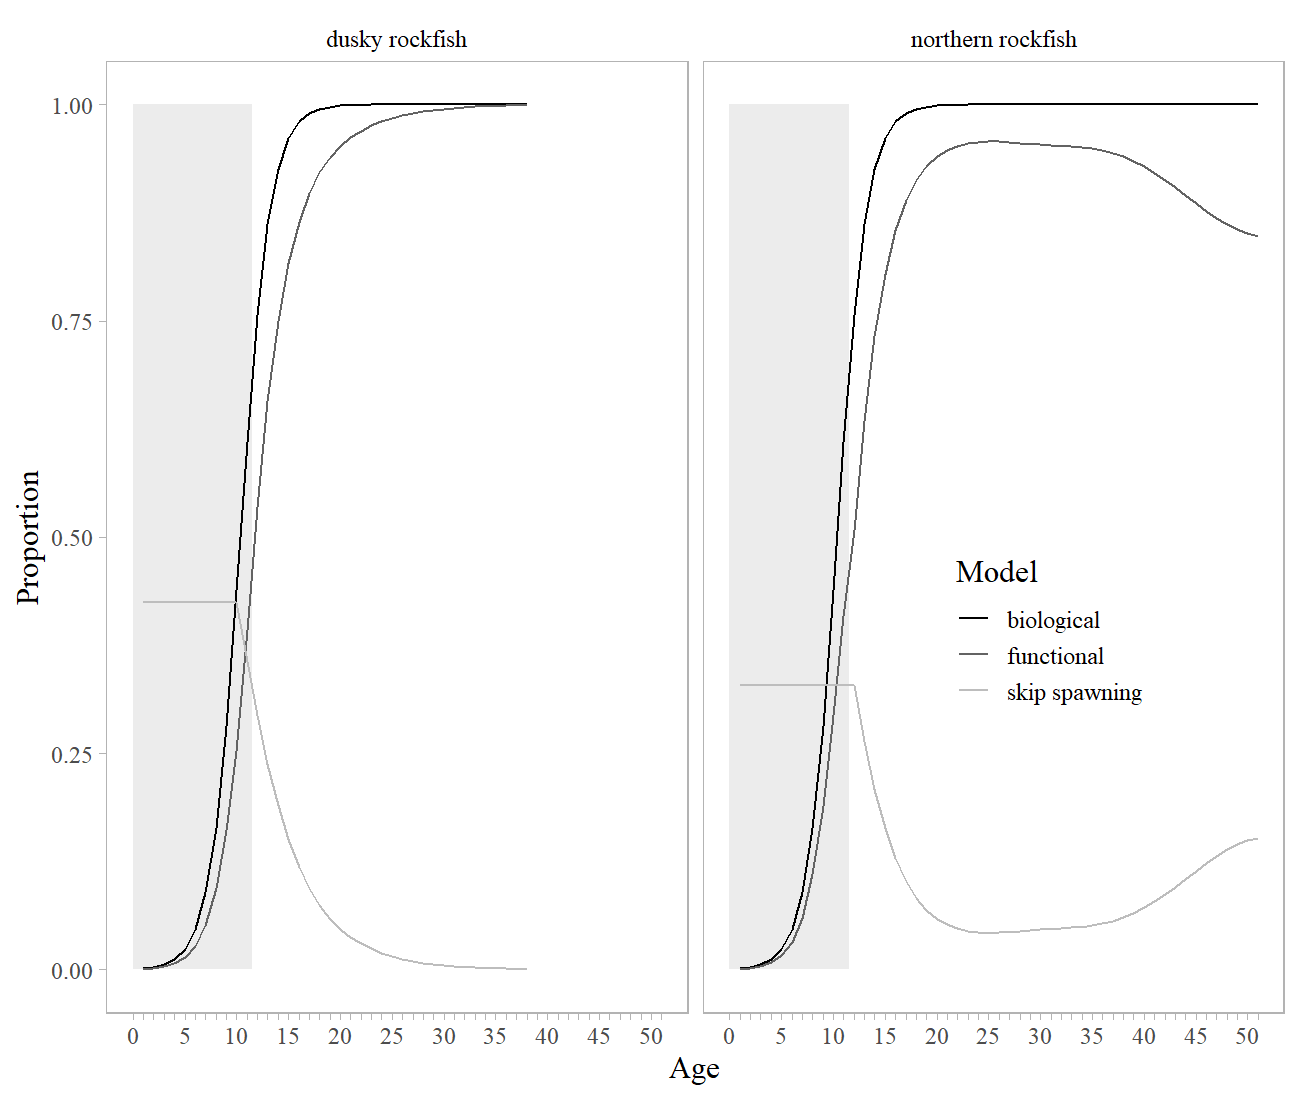
\includegraphics[width=5in,height=\textheight,keepaspectratio]{../figs/maturity.png}

}

\caption{\label{fig-maturity}The biological maturity ogive-at-age,
associated level of skip spawning and resultant functional maturity
ogive for Gulf of Alaska northern rockfish. The shaded box covers the
ages with no skip spawning information available.}

\end{figure}%

More AI slop

Simulation Results: Risk of Overfishing and Depletion Simulations were
conducted over a 100-year projection period to evaluate the stock's
response to full harvest allocations under three distinct recruitment
scenarios. Across all scenarios, the initial 10 to 20 years exhibit a
sharp decline in stock status, driving a high proportion of simulation
runs into ``Overfished'' or ``Critical'' categories. This early shock is
an expected artifact of the simulation transitioning from historical
realized catch levels (approximately 40\% of the Total Allowable Catch
{[}TAC{]}) to the assumption that 100\% of the TAC is fully harvested.

The simulations compare a ``Correct (Functional)'' model against a
``Misspecified (Biological)'' model, the latter representing an
assessment that fails to account for biological penalties (such as skip
spawning) and therefore overestimates stock resilience.

Scenario 1: Median Recruitment Under median recruitment conditions, the
stock experiences the initial full-TAC shock but begins to recover by
year 20 as the harvest control rule (HCR) restricts fishing mortality.

Correct (Functional): The correctly specified model recovers robustly,
with the probability of the stock remaining in the ``Safe'' category
staying between 75\% and 100\% for the remainder of the century.

Misspecified (Biological): While the misspecified model also shows
initial recovery, it exhibits a steady, long-term degradation in stock
status starting around year 40. By year 100, the probability of the
stock remaining ``Safe'' drops below 25\%, with the vast majority of
runs falling into the ``Buffer (ABC \textless{} F \textless{} OFL)''
category. This indicates that the misspecified HCR consistently fishes
the stock down below optimal target levels over the long term.

Scenario 2: 80th Percentile Recruitment This scenario tests the stock's
resilience under highly favorable, consistently above-average
recruitment. As expected, the high influx of recruits buffers the
initial full-TAC shock, resulting in a much narrower and shorter-lived
period of overfished status (resolving by year 15).

Correct (Functional): The stock easily sustains the maximum allowable
harvest, remaining overwhelmingly in the ``Safe'' category
(\textgreater75\% probability) for the entire 100-year series.

Misspecified (Biological): Remarkably, even under highly optimistic
recruitment assumptions, the misspecified model fails to maintain a
``Safe'' status. Similar to the median scenario, the proportion of
``Safe'' runs steadily declines after year 30, dropping to roughly 25\%
by year 100. The highly productive environment temporarily masks the
biological deficit, but the HCR's misspecified targets ultimately force
the stock to ride the threshold between the ``Safe'' and ``Buffer''
zones.

Scenario 3: 20-Year Recruitment Crash Followed by 80th Percentile This
stress-test scenario simulates a severe, two-decade recruitment failure
followed by a rapid shift to highly favorable conditions.

Both models show nearly 100\% of simulation runs falling into severe
``Overfished'' and ``Critical'' states for the first 35 years. The delay
in recovery highlights the biological maturity lag; even after high
recruitment resumes at year 20, it takes over a decade for those cohorts
to enter the spawning biomass and rescue the stock.

Correct (Functional): Once the mature recruits enter the fishery (around
year 35), the stock rapidly shifts through the ``Buffer'' zone and
stabilizes safely in the green zone from year 60 onward.

Misspecified (Biological): Following the delayed recovery at year 60,
the misspecified model immediately begins to erode again. By year 100,
the probability of the stock remaining ``Safe'' drops back down to
approximately 50\%, replaced entirely by the ``Buffer'' risk category.

Summary Takeaway Across all three recruitment scenarios, the biological
misspecification reliably leads to long-term stock degradation. While
favorable environmental conditions (80th percentile recruitment) can
temporarily mask the symptoms of overfishing and delay the decline, the
misspecified HCR consistently erodes the spawning stock biomass over a
multi-decadal timeline, pushing the fishery into heightened states of
risk regardless of recruitment strength.

\section{Discussion}\label{discussion}

repurcusions of ignoring skip spawning effects of inclusion of skip
spawning

AI slop below:

Steepness is arguably the most important---and the most notoriously
difficult to estimate---parameter in modern fisheries stock
assessments.While the compensation ratio (\(D\)) tells you the
multiplier of productivity near zero, steepness (always denoted as
\(h\)) puts that productivity into a standardized, practical
context.Here is how they connect and why steepness rules the assessment
world:1. What is Steepness (\(h\))?Steepness is officially defined as
the fraction of unfished recruitment (\(R_0\)) that is expected when the
spawning stock biomass is reduced to exactly 20\% of its unfished level
(\(0.2 S_0\)).If \(h = 1.0\): Recruitment is 100\% of \(R_0\) even when
the stock is knocked down to 20\%. The stock is incredibly resilient and
highly productive (essentially a flat line from \(S_0\) all the way down
to 20\%).If \(h = 0.2\): Recruitment drops linearly with spawning
biomass. At 20\% biomass, you get 20\% recruitment. There is zero
compensatory density dependence. If a fish has \(h=0.2\), almost any
commercial fishing will drive it toward collapse.For most marine fish,
steepness falls somewhere between \(0.4\) and \(0.9\).2. The Math
Translating \(D\) into \(h\)The relationship between \(D\) (the slope at
the origin) and \(h\) (steepness) depends on the specific shape of the
spawner-recruit model you are using. In the standard Beverton-Holt
model, the conversion is beautifully simple.To find steepness from the
compensation ratio:\[h = \frac{D}{D + 4}\]To find the compensation ratio
if you know steepness:\[D = \frac{4h}{1 - h}\]Example: If a stock has a
compensation ratio of \(D=4\) (meaning spawners are 4 times more
productive at low abundances), its steepness is \(h = 4/8\), or \(0.5\).
This means at 20\% spawning biomass, the stock will produce 50\% of its
unfished recruitment.3. Why is Steepness So Critical?If you are running
an assessment model, \(h\) acts as the ultimate dial for the stock's
biological resilience.It defines the Maximum Sustainable Yield (MSY):
You literally cannot calculate the true MSY, or the optimal fishing
mortality (\(F_{MSY}\)), without knowing steepness. Higher steepness
means a higher MSY and a higher allowable catch.It dictates rebuilding
times: If a stock is overfished, the steepness value will dictate how
many years it will take to rebuild to target levels.The ``Information
Void'': Here is the ultimate catch-22 in fisheries. To accurately
measure \(h\) with real data, you need data points showing what happens
when the stock is at 20\% of its unfished level. But management is
specifically designed to prevent the stock from ever getting that low.
Therefore, for well-managed stocks, you often lack the very data needed
to calculate steepness!Because steepness is so hard to estimate from a
noisy ``shotgun blast'' of data, scientists often have to fix the value
in the model based on life-history meta-analysis (e.g., assuming
\(h=0.7\) for a typical rockfish based on studies of similar
species).This circles us right back to your first question: because
\(h\) is so difficult to lock down, calculating absolute MSY is
incredibly uncertain, making SPR proxies the safest and most reliable
way to manage.Would you like to look at how we select specific SPR
targets (like \(30\%\) versus \(50\%\)) based on what we assume a
stock's steepness might be?

You are connecting the dots perfectly. Your intuition is exactly right:
skip spawning effectively decreases steepness (\(h\)), and it
fundamentally changes how you need to approach your SPR targets.When a
stock exhibits skip spawning---especially among younger, newly mature
fish---it creates a dangerous biological illusion if your management
framework isn't adjusted for it. Here is how skip spawning impacts
steepness and how you must adapt your SPR strategy to compensate.1. Why
Skip Spawning Decreases Steepness (\(h\))Remember that steepness (\(h\))
is a measure of resilience---the stock's ability to pump out recruits
when the population is knocked down to 20\% of its unfished level. This
relies entirely on the compensatory spike in productivity (\(D\)).If
young fish skip spawning (often because they are allocating their
limited energy to somatic growth or surviving poor environmental
conditions rather than gonadal development), the actual reproductive
engine of the stock is severely downgraded.At low population sizes, you
need every mature fish to produce eggs to achieve that compensatory
spike.If a massive chunk of your mature biomass is taking the year off,
the realized productivity per mature fish drops.A lower compensatory
ratio (\(D\)) mathematically results in a lower steepness (\(h\)). The
stock simply has less ``spring'' to bounce back from depletion.2. The
``Ghost Biomass'' Problem in SPRThe core of managing with SPR is
comparing your current Spawning Potential to your unfished Spawning
Potential.In traditional assessments, ``Spawning Stock Biomass'' (SSB)
is calculated by simply looking at weight-at-age and multiplying it by
maturity-at-age. But if you have skip spawning, a fish can be mature
(capable of spawning) but not active (actually dropping eggs this
year).If your SPR model counts these skip-spawners as part of the SSB,
you are managing based on ghost biomass. Your model will tell you that
you are at an SPR of 40\%, but because half your young fish aren't
actually spawning, the biological reality in the water might be an SPR
of 20\%. You will accidentally overfish the stock while the model tells
you everything is fine.

Options wher one cannot estimate MSY \& \(h\) Adjust the Denominator
(Use Fecundity, not Biomass): Instead of using mature female biomass to
calculate SPR, you must shift your SPR calculation to use Total Egg
Production (TEP) or active spawning biomass. This requires building a
``probability of spawning'' vector into your life-history tables
alongside the maturity vector. A 4-year-old fish might be 100\% mature,
but only have a 30\% probability of actually spawning.

Increase the SPR Target: If you cannot quantify the exact rate of skip
spawning to adjust the model's inner workings, you must manage the
uncertainty by shifting your proxy. Because skip spawning lowers
effective \(h\) (meaning the stock is less resilient than a standard
teleost), a generic SPR target of 30\% or 40\% is no longer safe. You
should treat the stock like a highly vulnerable species and shift your
management target to a more conservative proxy, such as an SPR of 50\%
or even 60\%.

\section{Conclusions}\label{conclusions}

Given the interaction between maturity-at-age (or length) estimation and
determination of biological reference points it would be prudent to
increase our understanding of the temporal and spatial consistency of
skip spawning for managed fisheries that exhibit skip spawning to some
degree. Further, a MSE approach, particularly a ``desktop'' MSE
\citep{Walter2023}

\section{Declaration of Competing
Interest}\label{declaration-of-competing-interest}

The author declares that he has no known competing financial interests
or personal relationships that could have appeared to influence the work
reported in this paper.

\section{Acknowledgements}\label{acknowledgements}

I thank Christina Conrath for providing maturity data for this analysis.
This research did not receive any specific grant from funding agencies
in the public, commercial, or not-for-profit sectors.

\section{Data Availability}\label{data-availability}

The data are available upon request from the author.

\section{References}\label{references}

\renewcommand{\bibsection}{}
\bibliography{references.bib}

\newpage{}

\section{Operating Model
Parameterization}\label{operating-model-parameterization}

{[}detailed tables of M, selectivity, and maturity ogives here.{]}

\section{Simulation Diagnostics}\label{simulation-diagnostics}

{[}convergence plots and trace plots for the 50 Monte Carlo iterations
here.{]}





\end{document}
